
\chapter{The BSP model, Pregel and Apache Spark}\label{r:pregel}
In the recent years, several models and many technologies that help efficiently perform iterative computations on large datasets, especially graphs, have been developed.

One of the most modern ones, Apache Spark, allows to express algorithms as transformations of RDDs, which are an abstraction of a distributed dataset. Its distinctive feature is that most of the data during the computation can be kept in worker nodes' memory, which gives makes it significantly faster than systems like Hadoop MapReduce. It is capable of handling wide range of tasks, including distributed graph computations using the GraphX extension.

Pregel is a computational model designed specifically for large graph computations, introduced in 2010 by Google engineers \cite{pregel}. Its goal is to streamline implementation of graph algorithms by providing a framework which lets the programmer forget about distributing the computation, implementing the graph topology and addressing fault tolerance issues and instead focus on the problem at hand. Pregel is based on the classical BSP model \cite{bsp} for iterative distributed computations.

Since introduction of Pregel, there have been many systems developed based on this model, most notably an open source implementation of the Pregel model, Apache Giraph. Pregel model of computations has also been incorporated into other, more general frameworks, including Spark. There have also been extensions to the model, such as Giraph++ \cite{giraphpp}.

Before Pregel and Spark, there were available graph algorithm libraries such as BGL \cite{bgl} and GraphBase \cite{GraphBase} which were designed for a single computer and thus limited in the scale of problems they could solve, and parallel graph frameworks such Parallel BGL \cite{parallelbgl}, which did not address issues crucial in large data processing, such as fault-tolerance. Graph algorithms also used to be expressed as a series of MapReduce iterations, but this adds a significant overhead due to the need to dump the state of computation to disk after each iteration, given that usually graph algorithms need multiple iterations.

In Section \ref{s:pregel}, the Pregel model is described. The RDD model used in Apache Spark and the Spark GraphX extension for graph computations, which supports the Pregel model, is covered in Section \ref{s:spark}.

\section{Pregel model and its original implementation}\label{s:pregel}

The name of the Pregel model comes from its initial proprietary implementation by Google and honors Leonard Euler, a famous Swiss mathematician and physicist and also a pioneer of the graph theory. In 1735, he formulated the first theorem in graph theory: a solution to an old question whether a Koenigsberg citizen could take a walk around the city so that he crossed each of the seven city's bridges exactly once. Euler concluded that it is impossible, because the graph bridges form is not what we today call an Euler graph --- a graph in which every vertex has an even degree. The name of river that flows through Koenigsberg and which the famous bridges spanned is Pregel.

The model of computation in Pregel is based on the L. Valiant's Bulk Synchronous Parallel model \cite{bsp}. The computation is performed in a sequence of \emph{supersteps}. In each superstep, the framework executes on each vertex a \emph{vertex program} provided by the user. Vertices communicate by messages: a message sent by a vertex in superstep $S$ is delivered to its recipient in superstep $S+1$. Figure \ref{bspiterimg} presents the phases in a single iteration of program execution in Pregel.

\begin{figure}[!htbp]
\centering
\begin{overpic}[width=0.8\textwidth,tics=10]{images/barriers.png}
 \put (60,57) {Vertices}
 \put (2,40) {Local computations}
 \put (2,18) {Communication}
 \put (2,6) {Synchronization}
\end{overpic}
\caption{One superstep in Pregel as a BSP iteration.\label{bspiterimg}}
\end{figure}

The main concept in implementing algorithms on Pregel is to "think like a vertex". User is required to express the algorithm as a function executed locally on each vertex, where communication between vertices is allowed only across supersteps. Those local functions are then combined by the framework in an efficient way to perform the whole computation. This approach, similar to the MapReduce model, is well suited for distributed computations, since all local functions can be executed in a fully independent way. At the same time, the synchronous structure of computation makes it easier to reason about the semantics of a program than in asynchronous systems and allows for fault-tolerance mechanisms.

A Pregel program takes a directed graph as an input and performs computations that are allowed to modify this graph.
Each vertex of the graph has a unique, constant \emph{vertex identifier} and is associated with some \emph{vertex data}, which can be modified during the computation. Vertex also has \emph{outgoing edges}, each of which has a target vertex and some modifiable \emph{edge data}. The algorithm logic is described using the \emph{vertex program}.

A computation is performed as a sequence of \emph{supersteps}. In each superstep the vertex program is concurrently executed on each vertex. The program is the same for each vertex, but can depend on the vertex identifier. The program executing on vertex $V$ receives messages sent to $V$ in the previous superstep. It can modify the vertex data and the data of its outgoing edges, send messages to other vertices to be delivered in the next superstep and change the topology of graph by adding or removing vertices or edges. A vertex can send messages not only to its neighbors, but also to other vertices if it knows their identifiers.

The termination criterion is distributed. A vertex may \emph{vote to halt}. Initially, all vertices are in the \emph{active} state. If a vertex votes to halt, its state changes to \emph{inactive}. If an inactive vertex receives a message from another vertex, it is moved back to the active state. The vertex program is executed only on the active vertices. The computation is terminated when all vertices are in the inactive state.

According to the original definition, the result of a computation are the values explicitly output by the vertices, but in most scenarios the graph state after the last superstep is assumed to be the output of the algorithm.

In practice, computations are performed on a number of workers much smaller than the number of vertices in the graph. This allows distributing the vertices between workers in a workload-balanced manner.

Let us consider the following example: for a strongly connected graph with an integer value assigned to each node, compute the minimum of those values. This can be implemented in Pregel using the vertex program presented on Figure \ref{psc:pregelmaxval}.

\begin{figure}[!htbp]

\begin{codebox}
  \Procname{$\proc{Max-Value-Vertex}(\textit{vertex, superstepNumber, incomingMessages})$}
  \li $\textit{newValue} \leftarrow \max\textit{incomingMessages} \cup \{\textit{vertex.value}\})$
  \li \If  $superstepNumber = 0$ \textbf{or} $\textit{newValue} > \textit{vertex.value}$
  \li \Then
   $\textit{vertex.value} \leftarrow \textit{newValue}$
   \li \textbf{foreach} $\textit{edge} \in \textit{vertex.outgoingEdges}$ \Then
  \li \proc{Send-Message}$(\textit{edge.targetVertex, newValue})$
  	  \End
  \li \Else
  \li \proc{Vote-To-Halt()}
      \End
\end{codebox}
\caption{Pregel vertex program for computing maximum value among graph nodes}\label{psc:pregelmaxval}
\end{figure}

In the first superstep, a vertex sends its value to all neighbors, and votes to halt. Upon reception of any new values, a vertex is activated and if the received values are greater than the value stored in the vertex, it is updated, and messages with the new value are sent. An example computation is presented on Figure \ref{img:pregelmaxval}. This picture comes from the original white paper about Pregel \cite{pregel}.

\begin{figure}[!ht]
\begin{center}
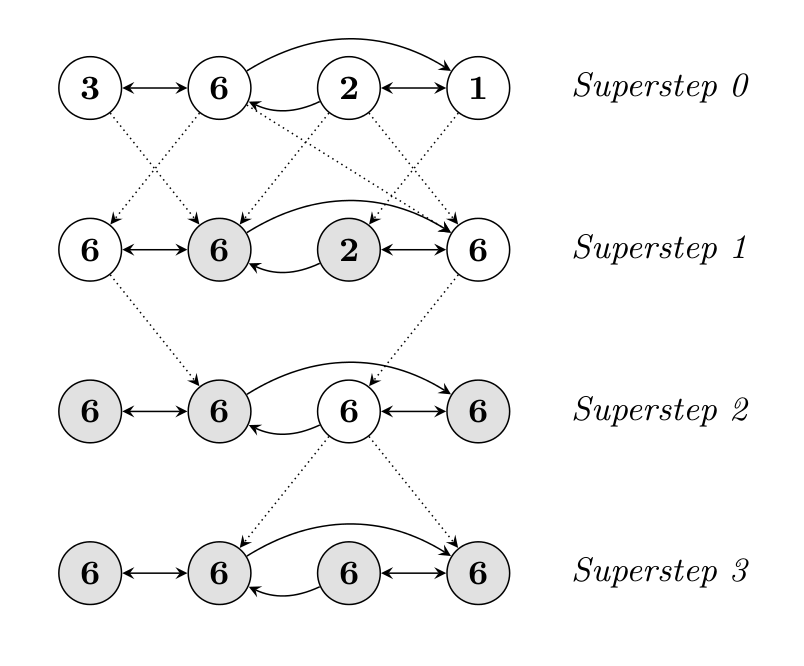
\includegraphics[width=0.6\textwidth]{PregelMaxVal.png}
\caption{Example Pregel computation of maximum value among the nodes. Nodes that voted to halt are marked gray. Source: \cite{pregel}}\label{img:pregelmaxval}
\end{center}
\end{figure}

For another example, let us see how single source shortest paths can be computed using Pregel. 
We assume that the value for each vertex is initially set to $\infty$.
In the first superstep the source vertex updates its value to $0$ and sends messages to its neighbors with a new distance. In the following supersteps
other vertices update their distances and, if it changed, send messages to their neighbors with a new possible distance. Each active vertex votes to halt in each superstep, so when no more messages with distance updates are sent, the algorithm terminates. This will always happen in a finite number of supersteps, as long as all edges have non-negative lengths. At the end of computation, each vertex has its minimum distance from \textit{SOURCE} associated with it, or $\infty$ if it is not reachable.

\begin{figure}[!htbp]
\begin{codebox}
  \Procname{$\proc{Shortest-Paths-Vertex}(\textit{vertex, superstepNumber, incomingMessages})$}
  \li $\textit{initialDistance} \leftarrow \textbf{if }(vertex.id = \textit{SOURCE})~0~\textbf{else}~\infty$
  \li $\textit{minDistance} \leftarrow \min(\textit{incomingMessages} \cup \{\textit{initialDistance}\})$
  \li \If $\textit{newValue} < \textit{vertex.value}$
  \li \Then
	  $\textit{vertex.value} \leftarrow \textit{minDistance}$
  \li \textbf{foreach} $\textit{edge} \in \textit{vertex.outgoingEdges}$ \Then
  \li \proc{Send-Message}$(\textit{edge.targetVertex, minDistance + edge.length})$
  	  \End
      \End
  \li \proc{Vote-To-Halt()}
\end{codebox}
\caption{Pregel vertex program for shortest paths from single source to all other vertices}
\end{figure}

An important goal in large dataset computations is to achieve fault-tolerance, so the computation can be continued in case of a failure of some of the machines in the cluster. In Pregel, this is achieved by \emph{checkpointing}. Once in a few supersteps, the workers are required to save their state to the disk. When any of the workers fails, the computation is resumed from the last checkpoint.

In addition to the general model, Pregel also has some additional features enhancing usability and efficiency, such as \emph{aggregators} for efficiently gathering and broadcasting global values and \emph{combiners} which can reduce the network bandwidth used by merging messages send from vertices placed on a given node.

The original implementation by Google engineers is proprietary and was never released to the public. It is written entirely in C++ and tightly connected to the internal Google infrastructure, including the distributed file systems and execution environment.

\subsection{Giraph}

Giraph \cite{giraph} is an open-source implementation of the Pregel model. It adds several extensions to the version originally described by Google. Those extensions include introducing the possibility to perform computations on the master node, capabilities to work with a support of external memory and removing the single point of failure by adding spare master nodes, which can become active when the primary master node fails.

Giraph is built on top of Hadoop \cite{hadoop}, the widely-adopted framework for large datasets processing. Hadoop is a platform for big datasets computing at scale, consisting of HDFS --- distributed file system, YARN --- framework for managing the cluster and scheduling tasks, Hadoop MapReduce --- an open implementation of the MapReduce model and libraries for using these elements in other projects.
 
Development of Giraph was started by Yahoo!. The project was donated to the Apache Foundation as an incubator project in 2011. It became a Top Level Project of the Apache Foundation in 2012. A stable version 1.0 was released in 2013. There are several large companies including Facebook, Twitter and LinkedIn using the project extensively and engaged in the development. The most active user is Facebook, which executes Giraph programs on social graphs with up to $10^{12}$ edges \cite{giraphfb}. In 2013 Facebook published an article \cite{giraphfb} stating that analyzing so large graphs was impossible with the software available in 2012. The article describes the optimizations and enhancements made in Giraph to be able to run jobs with this amount of data on their infrastructure:
\begin{itemize}
\item Flexible graph input: vertices and edges can be loaded from several sources and the framework takes care of distributing them correctly before the start of computation.
\item Multithreaded execution on a single machine, which allows for better resource sharing than in case of workers distributed across different machines.
\item Memory usage optimization: by serializing the transferred data using primitive types instead of Java objects, the memory usage was significantly reduced, resulting in 10 times lower execution time.
\item Sharded aggregators: instead of aggregators being stored and distributed by the master node, they are stored in a distributed way, which scales better for very large datasets.
\end{itemize}
It is worth mentioning that one of Google Pregel creators and the primary author of the original white paper about it, Grzegorz Malewicz, is one of the members of Facebook's data infrastructure graph processing team which develops Giraph \cite{giraphfb}.

\section{Spark}\label{s:spark}
Apache Spark \cite{spark, spark2} is an open-source framework for distributed data analytics. It started in 2009 in the AMPLab at University of California, Berkeley. Since that time it has gained a huge momentum and has quickly a growing community of users and contributors \cite{sparkgrowingcommunity}. Since 2009, over 250 individual developers contributed to Spark, and its permanent contributors come from 12 companies and institutions \cite{sparkwww}. Among others, it is being used by companies such as Yahoo, IBM, Intel, Alibaba, Cloudera and Databricks.

Spark's computational model is able to express programs in more specialized models such as MapReduce and Pregel and is also suitable for new applications that these systems do not support, like interactive data mining and stream data processing.

The two key advantages of Spark are:
\begin{itemize}
\item its impressive speed: Spark is in some cases even 100 times faster than equivalent computations in Hadoop MapReduce,
\item its simplicity and ease of use: it offers  APIs in Scala, Java, Python which allow developers to quickly develop programs performing even complicated calculations and a standalone running mode which lets developers set up environment and prototype programs locally without the need to set up Apache Hadoop.
\end{itemize}

Similarly to Apache Giraph, Spark is a Top-Level Project of the Apache Foundation. Previously to promotion as a Top-Level Project in February 2014 \cite{sparktoplevel}, it was in the Apache Incubator program since June 2013. 

Spark fits into the Hadoop ecosystem by being able to run on Hadoop clusters without any additional installation and supporting data input from various Hadoop data stores such as HDFS, HBase and Cassandra. It is not tied, however, to Hadoop infrastructure: it can also run as a standalone deployment in a cluster or on other distributed platforms such as Mesos \cite{mesos} and Amazon EC2 \cite{ec2}.

\subsection{Resilient Distributed Datasets}
The key concept in Spark is the \emph{Resilient Distributed Dataset} (RDD). RDDs are an abstraction of distributed memory, which let the programmer perform distributed computations. They are stored in a way that is transparent to the user and assures fault tolerance.

RDDs provide only a \emph{coarse-grained} interface: operations that are applied to the whole dataset, such as map, filter and join. This allows for achieving fault-tolerance by storing only the history of operations that were used to build a dataset, called its \emph{lineage}, instead of replicating the data to be able to recover it. An additional advantage is that the RDDs do not need to be materialized, unless it is actually necessary. Since parallel computations generally apply some transformation to multiple elements of a dataset, in most cases they can be expressed easily with coarse-grained operation on datasets.

RDDs can be created only in two ways: loading a dataset from a distributed storage or from another dataset by applying coarse-grained functional operations called \emph{transformations}, such as \emph{map}, \emph{filter} and \emph{join}. For greater efficiency, the user can also control the \emph{persistence} by indicating which RDDs are intended to be used in the future and as such should be materialized in the memory and the \emph{partitioning} of each RDD by indicating the key by which the records of RDD should be partitioned across the machines. Finally, the user can perform \emph{actions} on an RDD. Actions return a value or export the dataset to some persistent storage. Available actions include \emph{count}, which returns the number of elements in the RDD, \emph{collect}, which returns the records from the dataset and \emph{save}, which exports the records to an external storage.

\begin{exmp}
Let us suppose we have an RDD \emph{friends}, which consists of pairs of identifiers $(a, b)$ meaning that person $b$ is a friend of person $a$. We will say that $y$ is a \emph{friend of friend} of $x$ iff there exists $z$, called a \emph{proxy}, such that $z$ is a friend of $x$ and $y$ is a friend of $z$. We will call a person with more than 10000 friends of friends an \emph{influencer}. A Spark program which computes the number of all influencers is presented on Figure \ref{ex:sparkfof}.

\begin{figure}[!htbp]
\begin{codebox}
  \Procname{$\proc{Count-Influencers}(\textit{friends})$}
  \li $\textit{connections} \leftarrow \textit{friends}.\text{map}((x, y) \mapsto (y, x)).\text{join}(\textit{friends})$
  \li $\textit{friendsOfFriends} \leftarrow \textit{connections}.\text{map}((z, (x, y)) \mapsto (x, y)).distinct()$ 
  \li $\textit{fofCount} \leftarrow \textit{friendsOfFriends}.\text{map}((x, y) \mapsto (x, 1)).reduceByKey((m, n) \mapsto m+n)$
  \li $\textit{influencers} \leftarrow fofCount.filter((x, c) \mapsto count > 10000))$
  \li \Return $\textit{influencers}.\text{count}()$
\end{codebox}
\caption{Example of computation in Spark: computing the number influencers.}\label{ex:sparkfof}
\end{figure}

The \proc{Count-Influencers} function first performs a join of \emph{friends} with itself. Since the join transformation joins by the first value in the pair, the elements of \emph{friends} are swapped beforehand. The result is then mapped to remove the information about proxies, which is irrelevant, and duplicates are eliminated with \emph{distinct}. This gives an RDD of pairs $(x, y)$, such that $y$ is a friend of friend of $x$. For each $x$, the number of friends of friends is then computed using \emph{map} and \emph{reduceByKey}. The obtained RDD of pairs $(x, c)$, where $x$ is the person and $c$ is its number of friends of friends is then filtered so that only influencers remain. The size of the filtered RDD is returned as the number of influencers. It is worth noting that the used transformations \emph{map, filter, distinct} and \emph{reduceByKey} are not actually executed until the action \emph{count} is performed.

Iterative computation can be achieved in Spark by simply placing the transformations within a loop. For performance reasons, the user will often need to manage which RDDs should be cached in memory and explicitly materialize some of them in each iteration.
\end{exmp}

\subsection{Higher level tools}
Spark offers a set of high level tools that demonstrate the capabilities of the Resilient Distributed Dataset model. Those tools are implemented as relatively small libraries on top of Spark's core. Currently available tools are:
\begin{itemize}
\item Spark SQL, allowing seamless integration of SQL queries into Spark programs,
\item Spark Streaming, which supports working on on-line streams of data,
\item MLlib, which is an implementation of common machine learning algorithms for classification, regression, clustering and dimensionality reduction,
\item GraphX, providing an interface for creating efficient graph algorithms, integrated with pre- and post- processing with regular Spark transformations.
\end{itemize}

\section{Other frameworks}
Some of the other notable examples of systems designed for graph computations include the Graph Processing System, GraphLab and Giraph++.

Graph Processing System \cite{gps} is similar to Pregel and Giraph, but offers additional capabilities to express computations in a non-vertex-centric way, dynamically repartition vertices among workers based on their communication patterns and partitioning of adjacency lists of high-degree vertices. Giraph++ \cite{giraphpp} proposes a "think like a graph" model, as opposed to Pregel's "think like a vertex", to allow for algorithm-specific optimizations by giving more control over partitioning of data. In GraphLab \cite{graphlabwww, graphlab, graphlab2}, computations are expressed using \emph{update functions}, which modify vertices data and schedule further executions of update functions. This approach has several advantages, for example the ability to read the data in adjacent vertices other than by receiving a message from them, but can result in a large overhead due to scheduling.


